\section{Generación de señalamiento paso a paso}

	Inicialmente, el RNA ejecuta el Algoritmo \ref{alg:graph_network} (ver Sección \ref{sec:grafos}) para detectar todos los \textit{netElements}, sus coordenadas iniciales y finales en la topología, y el sentido en el que fueron definidas. Al concluir el Algoritmo \ref{alg:graph_network}, el RNA ejecuta el Algoritmo \ref{alg:connectedness} (ver Sección \ref{sec:grafos}) para analizar la conexidad de la red. El resultado obtenido se muestra en el Código \ref{lst:EJ6_1}, donde se describen las coordenadas de cada \textit{netElement} y se confirma que la red es conexa.
	
	\begin{lstlisting}[language = {}, caption = Detección de \textit{netElements} por parte del RNA , label = {lst:EJ6_1}]
	###### Starting Railway Network Analyzer #####
	Reading .railML file
	Creating railML object
	Analyzing railML object
	Analyzing graph
	ne1 [-1500, 450] [-600, 450] >>
	ne2 [-600, 450] [-300, 750] >> 
	ne3 [-600, 450] [300, 450] >>
	ne4 [300, 450] [1350, 750] >>
	ne5 [300, 450] [1200, 450] >>
	ne6 [-300, 750] [480, 750] >>
	ne7 [-300, 750] [1530, 1020] >>
	ne10 [1200, 450] [1950, 750] >>
	ne11 [1200, 450] [1950, 450] >>
	ne41 [1530, 1020] [2790, 1320] >>
	ne42 [1530, 1020] [390, 1260] <<
	The network is connected
	\end{lstlisting}
	
	Por ejemplo, el \textit{netElement} ne42 inicia en la coordenada (1530;1020) y finaliza en la coordenada (390;1260). El símbolo $<<$ indica que ne42 se encuentra definido de derecha a izquierda, ya que la componente x de la coordenada final es mayor a la de la coordenada inicial. En este caso la componente y es diferente en ambas coordenadas, ya que el \textit{netElement} ne42, tal como se aprecia en la Figura \ref{fig:EJ6_1}, es una curva.. Además, se puede comprobar que la lista obtenida en consistente con la Figura \ref{fig:EJ6_2}. Por ejemplo, ne1, ne2 y ne3 comparten la coordenada (-600;450), que coincide con la coordenada del cambio de vías Sw01.
	
	A continuación, el RNA detectará la infraestructura ferroviaria, las curvas peligrosas y los puntos medios de los netElements que el RNA considera demasiado largos. El análisis de la infraestructura se detalla en la Sección \ref{sec:bufferstop}, Sección \ref{sec:detectors}, Sección \ref{sec:platform} y Sección \ref{sec:crossing}, mientras que la detección de curvas y puntos medios se detalla en la Sección \ref{sec:tracks}. El RNA ejecuta el Algoritmo \ref{alg:switches_1}, Algoritmo \ref{alg:switches_2} y Algoritmo \ref{alg:switches_3} para confirmar la detección de cambios de vías simples, dobles y en tijeras. El resultado de este proceso se puede visualizar en el Código \ref{lst:EJ6_2}.
	
	\begin{lstlisting}[language = {}, caption = Detección de puntos críticos por parte del RNA , label = {lst:EJ6_2}]
	Analyzing infrastructure --> Infrastructure.RNA
	Detecting Danger --> Safe_points.RNA
	ne1 has a RailJoint[J01] @ [-1060, 450]
	ne3 has a Middle point @ [-375.0, 450]
	ne3 has a Middle point @ [-150.0, 450]
	ne3 has a Middle point @ [75.0, 450]
	ne4 has a Curve(2 lines) @ [[600, 750]]
	ne5 has a RailJoint[J06] @ [765, 450]
	ne6 has a Middle point @ [-40.0, 750]
	ne6 has a Middle point @ [220.0, 750]
	ne7 has a RailJoint[J01] @ [705, 1020]
	ne7 has a Curve(2 lines) @ [[-30, 1020]]
	ne10 has a Curve(2 lines) @ [[1500, 750]]
	ne11 has a RailJoint[J02] @ [1653, 450]
	ne41 has a Curve(3 lines) @ [[1950, 1020], [2250, 1320]]
	ne42 has a Curve(2 lines) @ [[1290, 1260]]
	\end{lstlisting}
	
	Esta información es exportada por el RNA, con mayor detalle, en el archivo Infrastructure.RNA (Código \ref{lst:EJ6_4}) que resume cada elemento ferroviario asociado a su respectivo \textit{netElement}.
	
	\begin{lstlisting}[language = {}, caption = Infrastructure.RNA, label = {lst:EJ6_4}]
Nodes: 11|Switches: 5|Signals: 0|Detectors: 4|Ends: 7|Barriers: 0
Node ne1:
	Track = track1
	TrainDetectionElements -> tde16
		Type -> insulatedRailJoint
	Neighbours = 2 -> ['ne3', 'ne2']
	Switches -> Sw01
		ContinueCourse -> right -> ne3
		BranchCourse -> left -> ne2
Node ne2:
	Track = track7
	Neighbours = 4 -> ['ne1', 'ne3', 'ne7', 'ne6']
	Switches -> Sw03
		ContinueCourse -> left -> ne7
		BranchCourse -> right -> ne6
Node ne3:
	Track = track6
	Neighbours = 4 -> ['ne1', 'ne2', 'ne5', 'ne4']
	Switches -> Sw02
		ContinueCourse -> right -> ne5
		BranchCourse -> left -> ne4
Node ne4:
	Track = track5
	Type = BufferStop -> ['bus15']
	Neighbours = 2 -> ['ne3', 'ne5']
Node ne5:
	Track = track8
	TrainDetectionElements -> tde25
		Type -> insulatedRailJoint
	Neighbours = 4 -> ['ne3', 'ne4', 'ne10', 'ne11']
	Switches -> Sw05
		ContinueCourse -> right -> ne11
		BranchCourse -> left -> ne10
Node ne6:
	Track = track4
	Type = BufferStop -> ['bus14']
	Neighbours = 2 -> ['ne2', 'ne7']
Node ne7:
	Track = track9
	TrainDetectionElements -> tde67
		Type -> insulatedRailJoint
	Neighbours = 4 -> ['ne2', 'ne6', 'ne41', 'ne42']
Node ne10:
	Track = track3
	Type = BufferStop -> ['bus7']
	Neighbours = 2 -> ['ne5', 'ne11']
Node ne11:
	Track = track2
	TrainDetectionElements -> tde21
		Type -> insulatedRailJoint
	Neighbours = 2 -> ['ne5', 'ne10']
Node ne41:
	Track = track10
	Type = BufferStop -> ['bus62']
	Neighbours = 2 -> ['ne7', 'ne42']
	Switches -> Sw08
		ContinueCourse -> left -> ne7
		BranchCourse -> right -> ne42
Node ne42:
	Track = track11
	Type = BufferStop -> ['bus66']
	Neighbours = 2 -> ['ne7', 'ne41']
	\end{lstlisting}
	
	La información de la infraestructura es utilizada por el RNA para detectar los puntos críticos de la red, es decir, las zonas donde es recomendable colocar una señal, según el sentido de circulación que se desee. El resultado es exportado al archivo SafePoints.RNA (Código \ref{lst:EJ6_5}). En el caso de que un mismo \textit{netElement} tenga más de un punto crítico para el mismo sentido, el RNA tomará el más cercano al elemento a proteger. El criterio de selección de puntos críticos se aplica para cada elemento ferroviario detectado, cada curva y cada cambio de vías y fue explicado en las secciones correspondientes ya mencionadas.
	
	\begin{lstlisting}[language = {}, caption = SafePoints.RNA, label = {lst:EJ6_5}]
ne1:
	Next: [[-1160.0, 450]]
	Prev: [[-960.0, 450]]
ne3:
	Next: [[-375.0, 450], [-150.0, 450], [75.0, 450]]
	Prev: [[-375.0, 450], [-150.0, 450], [75.0, 450]]
ne4:
	Prev: [[700.0, 750]]
ne5:
	Next: [[665.0, 450]]
	Prev: [[865.0, 450]]
ne6:
	Next: [[-40.0, 750], [220.0, 750]]
	Prev: [[-40.0, 750], [220.0, 750]]
ne7:
	Next: [[605.0, 1020]]
	Prev: [[805.0, 1020], [70.0, 1020]]
ne10:
	Prev: [[1600.0, 750]]
ne11:
	Next: [[1553.0, 450]]
	Prev: [[1753.0, 450]]
ne41:
	Next: [[1850.0, 1020]]
	Prev: [[2350.0, 1320]]
ne42:
	Next: [[1190.0, 1260]]
	\end{lstlisting}	
	
	Una vez que el RNA detectó cada punto crítico de la red ferroviaria, procede a generar el señalamiento. El orden en que se procesan los elementos ferroviarios no impacta en el resultado final, pero para poder describirlo de forma ordenada se iniciará generando el señalamiento para proteger los finales de vías, las junturas entre rieles, las plataformas (explicado en la Sección \ref{sec:sig_platform}), los cruces de vía (explicado en la Sección \ref{sec:sig_levelcrossing}) y los cambios de vías (explicado en la Sección \ref{sec:signal_switches}). Luego se procederá a mostrar el señalamiento completo antes y después de la simplificación de señales (explicado en la Sección \ref{sec:simplificacion}). 
	
	Tal cómo se explicó en la Sección \ref{sec:sig_border}, el RNA aplica el Algoritmo \ref{alg:lineBorder} y el Algoritmo \ref{alg:bufferStop} para generar las señales para proteger los finales de vías relativos y absolutos. Estas señales son ilustradas en la Figura \ref{fig:EJ6_3}.
	
	\begin{figure}[H]
		\centering
		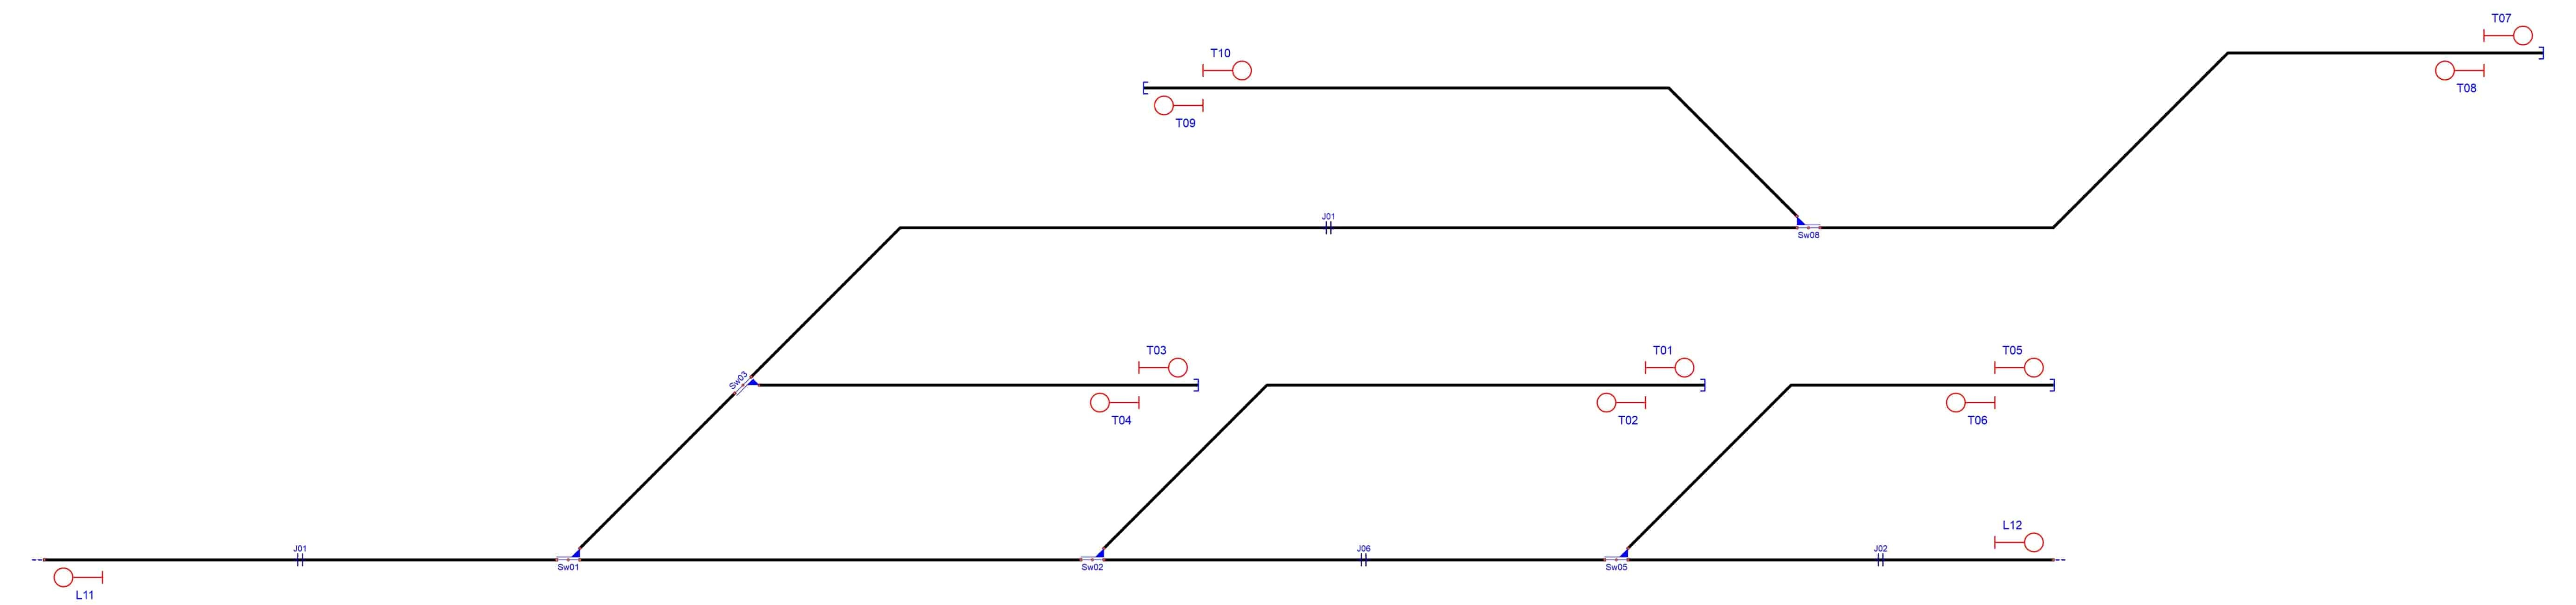
\includegraphics[width=1\textwidth]{resultados-obtenidos/ejemplo6/images/6_step1.png}
		\centering\caption{Señalamiento generado por el RNA para proteger el fín de vía.}
		\label{fig:EJ6_3}
	\end{figure}

	Los finales de vías absolutos son protegidos por las señales de parada T01, T03, T05, T07 y T09; y las señales de partida son T02, T04, T06, T08 y T10. A su vez, los finales de vías relativos poseen las señales de parada L11 y L12, cercanos al límite del externo del \textit{netElement} al que pertenecen.
	
	La Figura \ref{fig:EJ6_3} ilustra la generación de señales destinadas a proteger las junturas entre los rieles. Estas señales se obtuvieron al aplicar el Algoritmo \ref{alg:RJ}, tal como fue explicado en la Sección \ref{sec:sig_joint}. Las señales generadas son todas las señales comprendidas entre J13 y J20, indicadas en color rojo.

	\begin{figure}[H]
		\centering
		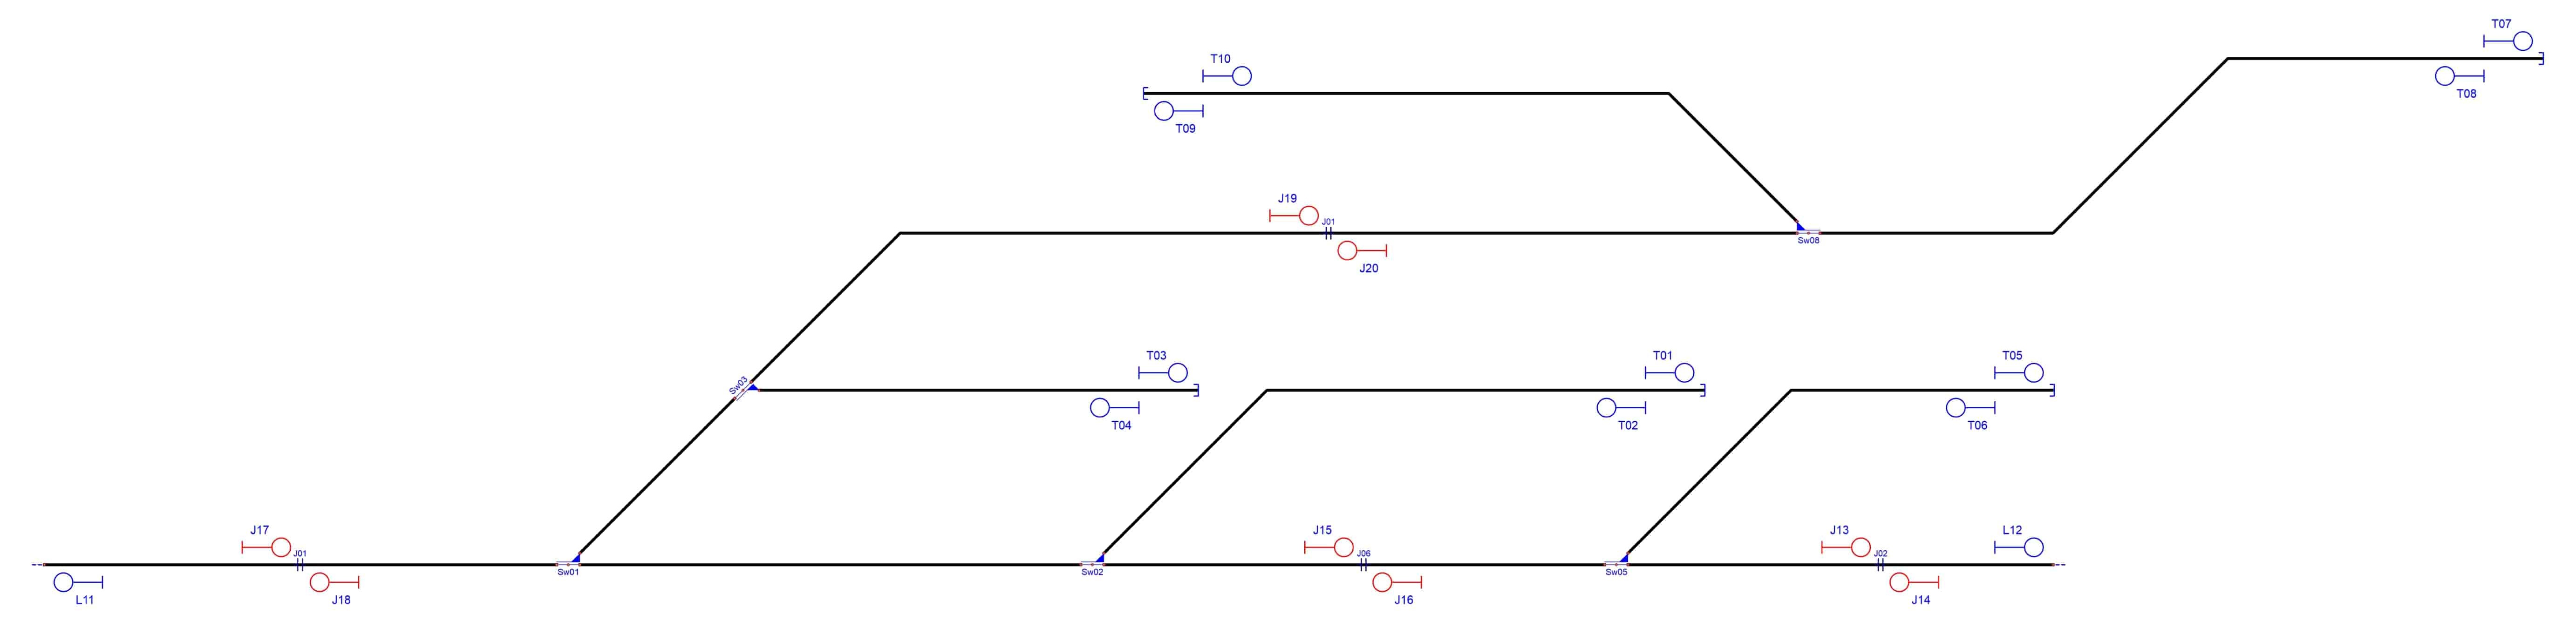
\includegraphics[width=1\textwidth]{resultados-obtenidos/ejemplo6/images/6_step2.png}
		\centering\caption{Señalamiento generado por el RNA para proteger las junturas.}
		\label{fig:EJ6_4}
	\end{figure}
	
	Al generar el señalamiento para proteger la infraestructura, tal como se explicó en la Sección \ref{sec:horizontal}, el Algoritmo \ref{alg:horizontal} simplificará las señales entre dos elementos ferroviarios si no existe espacio suficiente entre ellos. En este ejemplo, no existen plataformas o cruces de vías que proteger. Por lo tanto, el RNA no asigna nuevo señalamiento, como se visualiza en la Figura \ref{fig:EJ6_5}.

	\begin{figure}[H]
		\centering
		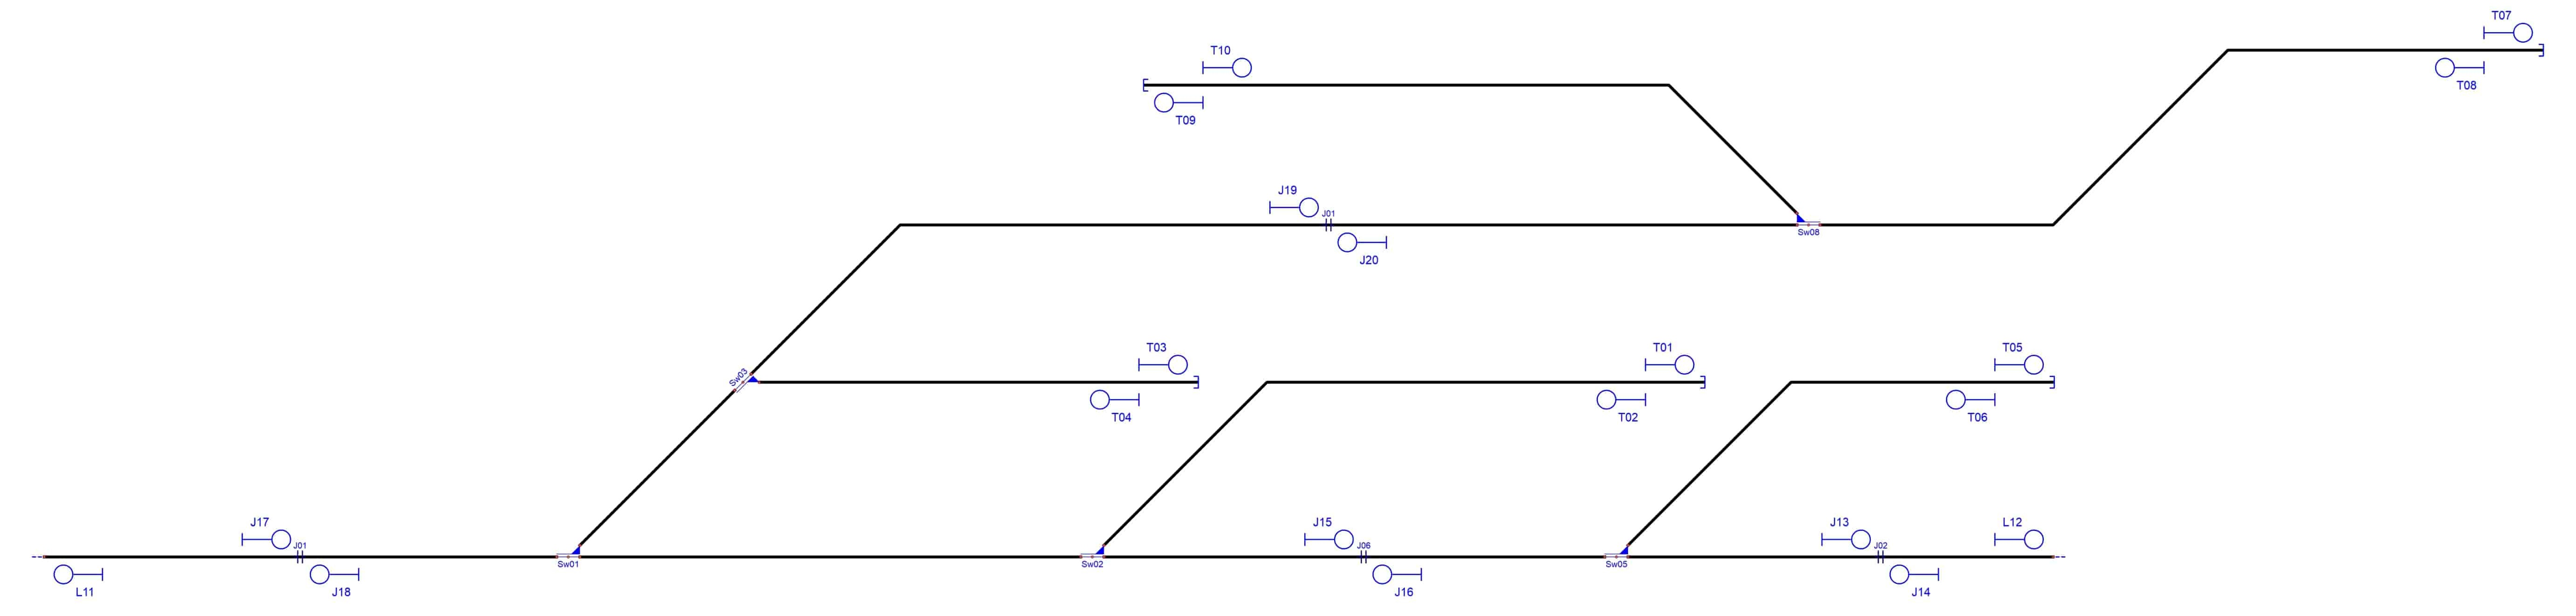
\includegraphics[width=1\textwidth]{resultados-obtenidos/ejemplo6/images/6_step3.png}
		\centering\caption{Señalamiento generado por el RNA para proteger plataformas y cruces de vía.}
		\label{fig:EJ6_5}
	\end{figure}

	Al aplicar el Algoritmo \ref{alg:SW} de generación de señalamiento para cambios de vías, tal como fue explicado en la Sección \label{sec:signal_switches}, el RNA genera las señales C21, S22 y H23 para proteger el cambio de vías Sw01; las señales C25, S27, B26 y H28 para proteger el cambio de vías Sw02; las señales C29, B30 Y H24 para proteger el cambio de vías Sw03; las señales C31, S33, B32 y H34 para proteger el cambio de vías Sw05 y las señales C35, S37, B36 y H38 para proteger el cambio de vías Sw08. Las señales mencionadas se encuentran resaltadas en rojo en la Figura \ref{fig:EJ6_6}.
	
	 \begin{figure}[H]
		\centering
		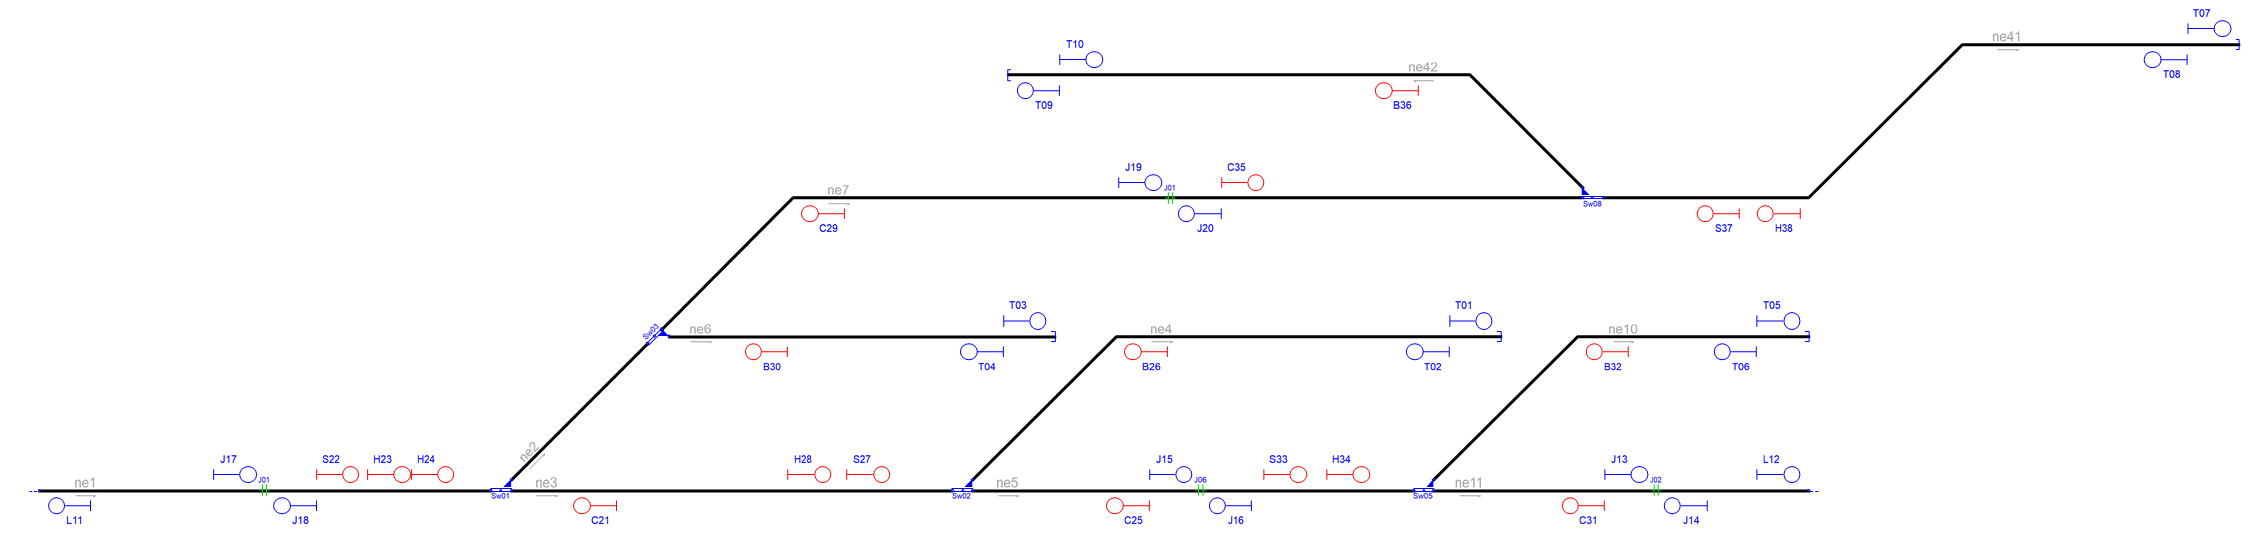
\includegraphics[width=1\textwidth]{resultados-obtenidos/ejemplo6/images/6_step4.png}
		\centering\caption{Señalamiento generado por el RNA para proteger las máquinas de cambios.}
		\label{fig:EJ6_6}
	\end{figure}
	
	Una vez obtenido todo el señalamiento, el RNA procede a simplificar las señales redundantes, repetidas o cuyas funciones o ubicaciones se superponen entre sí. El proceso de simplificación de señales fue explicado en la Sección \ref{sec:simplificacion}. El Algoritmo \ref{alg:vertical} de herencia vertical fue aplicado en la señal B del cambio de vías Sw01, moviéndola hasta la señal C29 del cambio de vías Sw03. Además, la señal S del cambio de vías Sw03 fue movida a la señal H23 del cambio de vías Sw01.
	
	Las señales simplificadas al aplicar el Algoritmo \ref{alg:horizontal} de herencia horizontal son: L12, J15, J17, H23, H24, C25, H28, B30, C31, B32, H34, C35 y H38. La señal H23 fue eliminada por su cercanía con la señal S22, con la cual comparten dirección y sentido. Lo mismo ocurre entre las señales H24 y S22; entre las señales H28 y S27; entre las señales H34 y S33; y entre las señales H38 y S37. En todos los casos, se aplicó el Algoritmo \ref{alg:horizontal}, diseñado para agrupar objetos cercanos como un único objeto, generando el señalamiento acorde a los elementos contenidos en cada extremo del nuevo elemento contenedor.
	
	Finalmente, las señales son simplificadas aplicando el Algoritmo \ref{alg:reduction} de eliminación por prioridad de señales. El resultado de este proceso es detallado en el Código \ref{lst:EJ6_3}.
	
	\begin{lstlisting}[language = {}, caption = Reducción de señalamiento por prioridad de señales, label = {lst:EJ6_3}]
	Reducing redundant signals
	T priority removing sig30 for sig04
	T priority removing sig32 for sig06
	L priority removing sig12 for sig13
	J>H priority removing sig31 for sig14
	J>S priority removing sig15 for sig33
	J>H priority removing sig25 for sig16
	J>S priority removing sig17 for sig22
	J>H priority removing sig35 for sig19
	Same position removing sig23 for sig22
	Same position removing sig24 for sig22
	Same position removing sig28 for sig27
	Same position removing sig34 for sig33
	Same position removing sig38 for sig37
	\end{lstlisting}

	El resultado de la simplificación del señalamiento se ilustra en la Figura \ref{fig:EJ6_7}.
	
	 \begin{figure}[H]
		\centering
		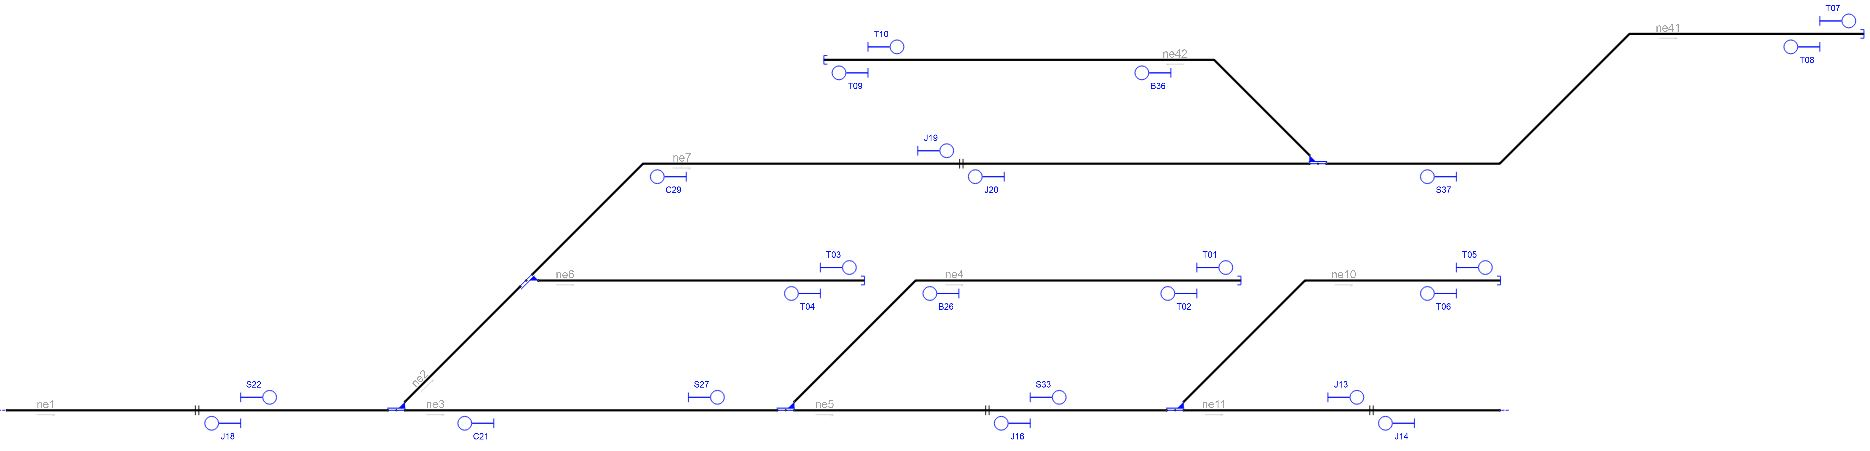
\includegraphics[width=1\textwidth]{resultados-obtenidos/ejemplo6/images/6_RNA.png}
		\centering\caption{Señalamiento generado y simplificado por el RNA.}
		\label{fig:EJ6_7}
	\end{figure}

	Además, toda la información del señalamiento generado es exportada por el RNA en el archivo Signalling.RNA (Código \ref{lst:EJ1_6}), que incluye información detallada de la posición, orientación, sentido, coordenada, nombre y tipo de señal.
	
	\begin{lstlisting}[language = {}, caption = Signalling.RNA, label = {lst:EJ6_6}]
sig01 [T01] >>:
	From: ne4 | To: bus15_right
	Type: Stop | Direction: normal | AtTrack: left 
	Position: [1250, -750] | Coordinate: 0.9148
sig02 [T02] <<:
	From: ne4 | To: ne4_left
	Type: Stop | Direction: reverse | AtTrack: right 
	Position: [1250, -750] | Coordinate: 0.9148
sig03 [T03] >>:
	From: ne6 | To: bus14_right
	Type: Stop | Direction: normal | AtTrack: left 
	Position: [380, -750] | Coordinate: 0.8717
sig04 [T04] <<:
	From: ne6 | To: ne6_left
	Type: Stop | Direction: reverse | AtTrack: right 
	Position: [380, -750] | Coordinate: 0.8717
sig05 [T05] >>:
	From: ne10 | To: bus7_right
	Type: Stop | Direction: normal | AtTrack: left 
	Position: [1850, -750] | Coordinate: 0.8856
sig06 [T06] <<:
	From: ne10 | To: ne10_left
	Type: Stop | Direction: reverse | AtTrack: right 
	Position: [1850, -750] | Coordinate: 0.8856
sig07 [T07] >>:
	From: ne41 | To: bus62_right
	Type: Stop | Direction: normal | AtTrack: left 
	Position: [2690, -1320] | Coordinate: 0.9277
sig08 [T08] <<:
	From: ne41 | To: ne41_left
	Type: Stop | Direction: reverse | AtTrack: right 
	Position: [2690, -1320] | Coordinate: 0.9277
sig09 [T09] <<:
	From: ne42 | To: bus66_left
	Type: Stop | Direction: normal | AtTrack: left 
	Position: [490, -1260] | Coordinate: 0.3545
sig10 [T10] >>:
	From: ne42 | To: ne42_right
	Type: Stop | Direction: reverse | AtTrack: right 
	Position: [490, -1260] | Coordinate: 0.3545
sig13 [J13] >>:
	From: ne11 | To: ne11_right
	Type: Circulation | Direction: normal | AtTrack: left 
	Position: [1553.0, -450] | Coordinate: 0.4706
sig14 [J14] <<:
	From: ne11 | To: ne11_left
	Type: Circulation | Direction: reverse | AtTrack: right 
	Position: [1753.0, -450] | Coordinate: 0.7373
sig16 [J16] <<:
	From: ne5 | To: ne5_left
	Type: Circulation | Direction: reverse | AtTrack: right 
	Position: [865.0, -450] | Coordinate: 0.6277
sig18 [J18] <<:
	From: ne1 | To: ne1_left
	Type: Circulation | Direction: reverse | AtTrack: right 
	Position: [-960.0, -450] | Coordinate: 0.6
sig19 [J19] >>:
	From: ne7 | To: ne7_right
	Type: Circulation | Direction: normal | AtTrack: left 
	Position: [605.0, -1020] | Coordinate: 0.5236
sig20 [J20] <<:
	From: ne7 | To: ne7_left
	Type: Circulation | Direction: reverse | AtTrack: right 
	Position: [805.0, -1020] | Coordinate: 0.6266
sig21 [C21] <<:
	From: ne3 | To: ne3_left
	Type: Circulation | Direction: reverse | AtTrack: right 
	Position: [-375.0, -450] | Coordinate: 0.25
sig22 [S22] >>:
	From: ne1 | To: ne1_right
	Type: Circulation | Direction: normal | AtTrack: left 
	Position: [-960.0, -450] | Coordinate: 0.6
sig26 [B26] <<:
	From: ne4 | To: ne4_left
	Type: Manouver | Direction: reverse | AtTrack: right 
	Position: [700.0, -750] | Coordinate: 0.4464
sig27 [S27] >>:
	From: ne3 | To: ne3_right
	Type: Circulation | Direction: normal | AtTrack: left 
	Position: [75.0, -450] | Coordinate: 0.75
sig29 [C29] <<:
	From: ne7 | To: ne7_left
	Type: Manouver | Direction: reverse | AtTrack: right 
	Position: [70.0, -1020] | Coordinate: 0.2481
sig33 [S33] >>:
	From: ne5 | To: ne5_right
	Type: Circulation | Direction: normal | AtTrack: left 
	Position: [865.0, -450] | Coordinate: 0.6277
sig36 [B36] <<:
	From: ne42 | To: ne42_right
	Type: Manouver | Direction: normal | AtTrack: left 
	Position: [1190.0, -1260] | Coordinate: 0.9193
sig37 [S37] <<:
	From: ne41 | To: ne41_left
	Type: Circulation | Direction: reverse | AtTrack: right 
	Position: [1850.0, -1020] | Coordinate: 0.9277
	\end{lstlisting}
	
	Al finalizar la generación del señalamiento, el RNA ejecuta el Algoritmo \ref{alg:routes}, explicado en la Sección \ref{sec:rutas}, para detectar todas las posibles rutas admitidas por la red para crear la tabla de enclavamientos. La cuál puede ser visualizada en el archivo Routes.RNA (Código \ref{lst:EJ6_7}). La misma detalla las señales de inicio y final, los \textit{netElements} abarcados por la ruta y cualquier infraestructura involucrada, incluyendo el estado que deben tener para que la ruta sea activada.
	
	\begin{lstlisting}[language = {}, caption = Routes.RNA, label = {lst:EJ6_7}]
route_1 [sig02 << sig26]:
	Path: ['ne4']
route_2 [sig04 << sig18]:
	Path: ['ne6', 'ne2', 'ne1']
	Switches: ['Sw01', 'Sw03']
route_3 [sig06 << sig16]:
	Path: ['ne10', 'ne5']
	Switches: ['Sw05']
route_4 [sig08 << sig37]:
	Path: ['ne41']
	Switches: ['Sw08']
route_5 [sig10 >> sig07]:
	Path: ['ne42', 'ne41']
	Switches: ['Sw08']
route_6 [sig14 << sig16]:
	Path: ['ne11', 'ne5']
	Switches: ['Sw05']
route_7 [sig16 << sig21]:
	Path: ['ne5', 'ne3']
	Switches: ['Sw02', 'Sw05']
route_8 [sig19 >> sig07]:
	Path: ['ne7', 'ne41']
	Switches: ['Sw08']
route_9 [sig20 << sig29]:
	Path: ['ne7']
route_10 [sig21 << sig18]:
	Path: ['ne3', 'ne1']
	Switches: ['Sw01', 'Sw02']
route_11 [sig22 >> sig27]:
	Path: ['ne1', 'ne3']
	Switches: ['Sw01', 'Sw02']
route_12 [sig22 >> sig19]:
	Path: ['ne1', 'ne2', 'ne7']
	Switches: ['Sw01', 'Sw03']
route_13 [sig22 >> sig03]:
	Path: ['ne1', 'ne2', 'ne6']
	Switches: ['Sw01', 'Sw03']
route_14 [sig26 << sig21]:
	Path: ['ne4', 'ne3']
	Switches: ['Sw02']
route_15 [sig27 >> sig33]:
	Path: ['ne3', 'ne5']
	Switches: ['Sw02', 'Sw05']
route_16 [sig27 >> sig01]:
	Path: ['ne3', 'ne4']
	Switches: ['Sw02']
route_17 [sig29 << sig18]:
	Path: ['ne7', 'ne2', 'ne1']
	Switches: ['Sw01', 'Sw03']
route_18 [sig33 >> sig05]:
	Path: ['ne5', 'ne10']
	Switches: ['Sw05']
route_19 [sig33 >> sig13]:
	Path: ['ne5', 'ne11']
	Switches: ['Sw05']
route_20 [sig36 << sig09]:
	Path: ['ne42']
route_21 [sig37 << sig20]:
	Path: ['ne41', 'ne7']
	Switches: ['Sw08']
route_22 [sig37 << sig36]:
	Path: ['ne41', 'ne42']
	Switches: ['Sw08']
	\end{lstlisting}
	
	
	
	
	
		